\section{Discussion}

Throughout the process of implementing the compiler and simulator for the CRN++ language, we discovered multiple times that not all chemical reactions worked as expected and that certain restrictions applied which were not listed in the paper \cite{soloveichik2018a}. Most notably, we found that the reactions for the \texttt{sqrt} module consistently calculate the fourth root instead of as expected the square root (see figure \ref{fig:subfigure1}). One example for a further restriction we discovered was that the input species to the \texttt{mul} module have to be different. If they are the same, the module produces $a^4$ instead of $a^2$ (see figure \ref{fig:subfigure2}). 

\begin{figure}[h]
  \centering
  \begin{subfigure}[b]{0.49\textwidth}
    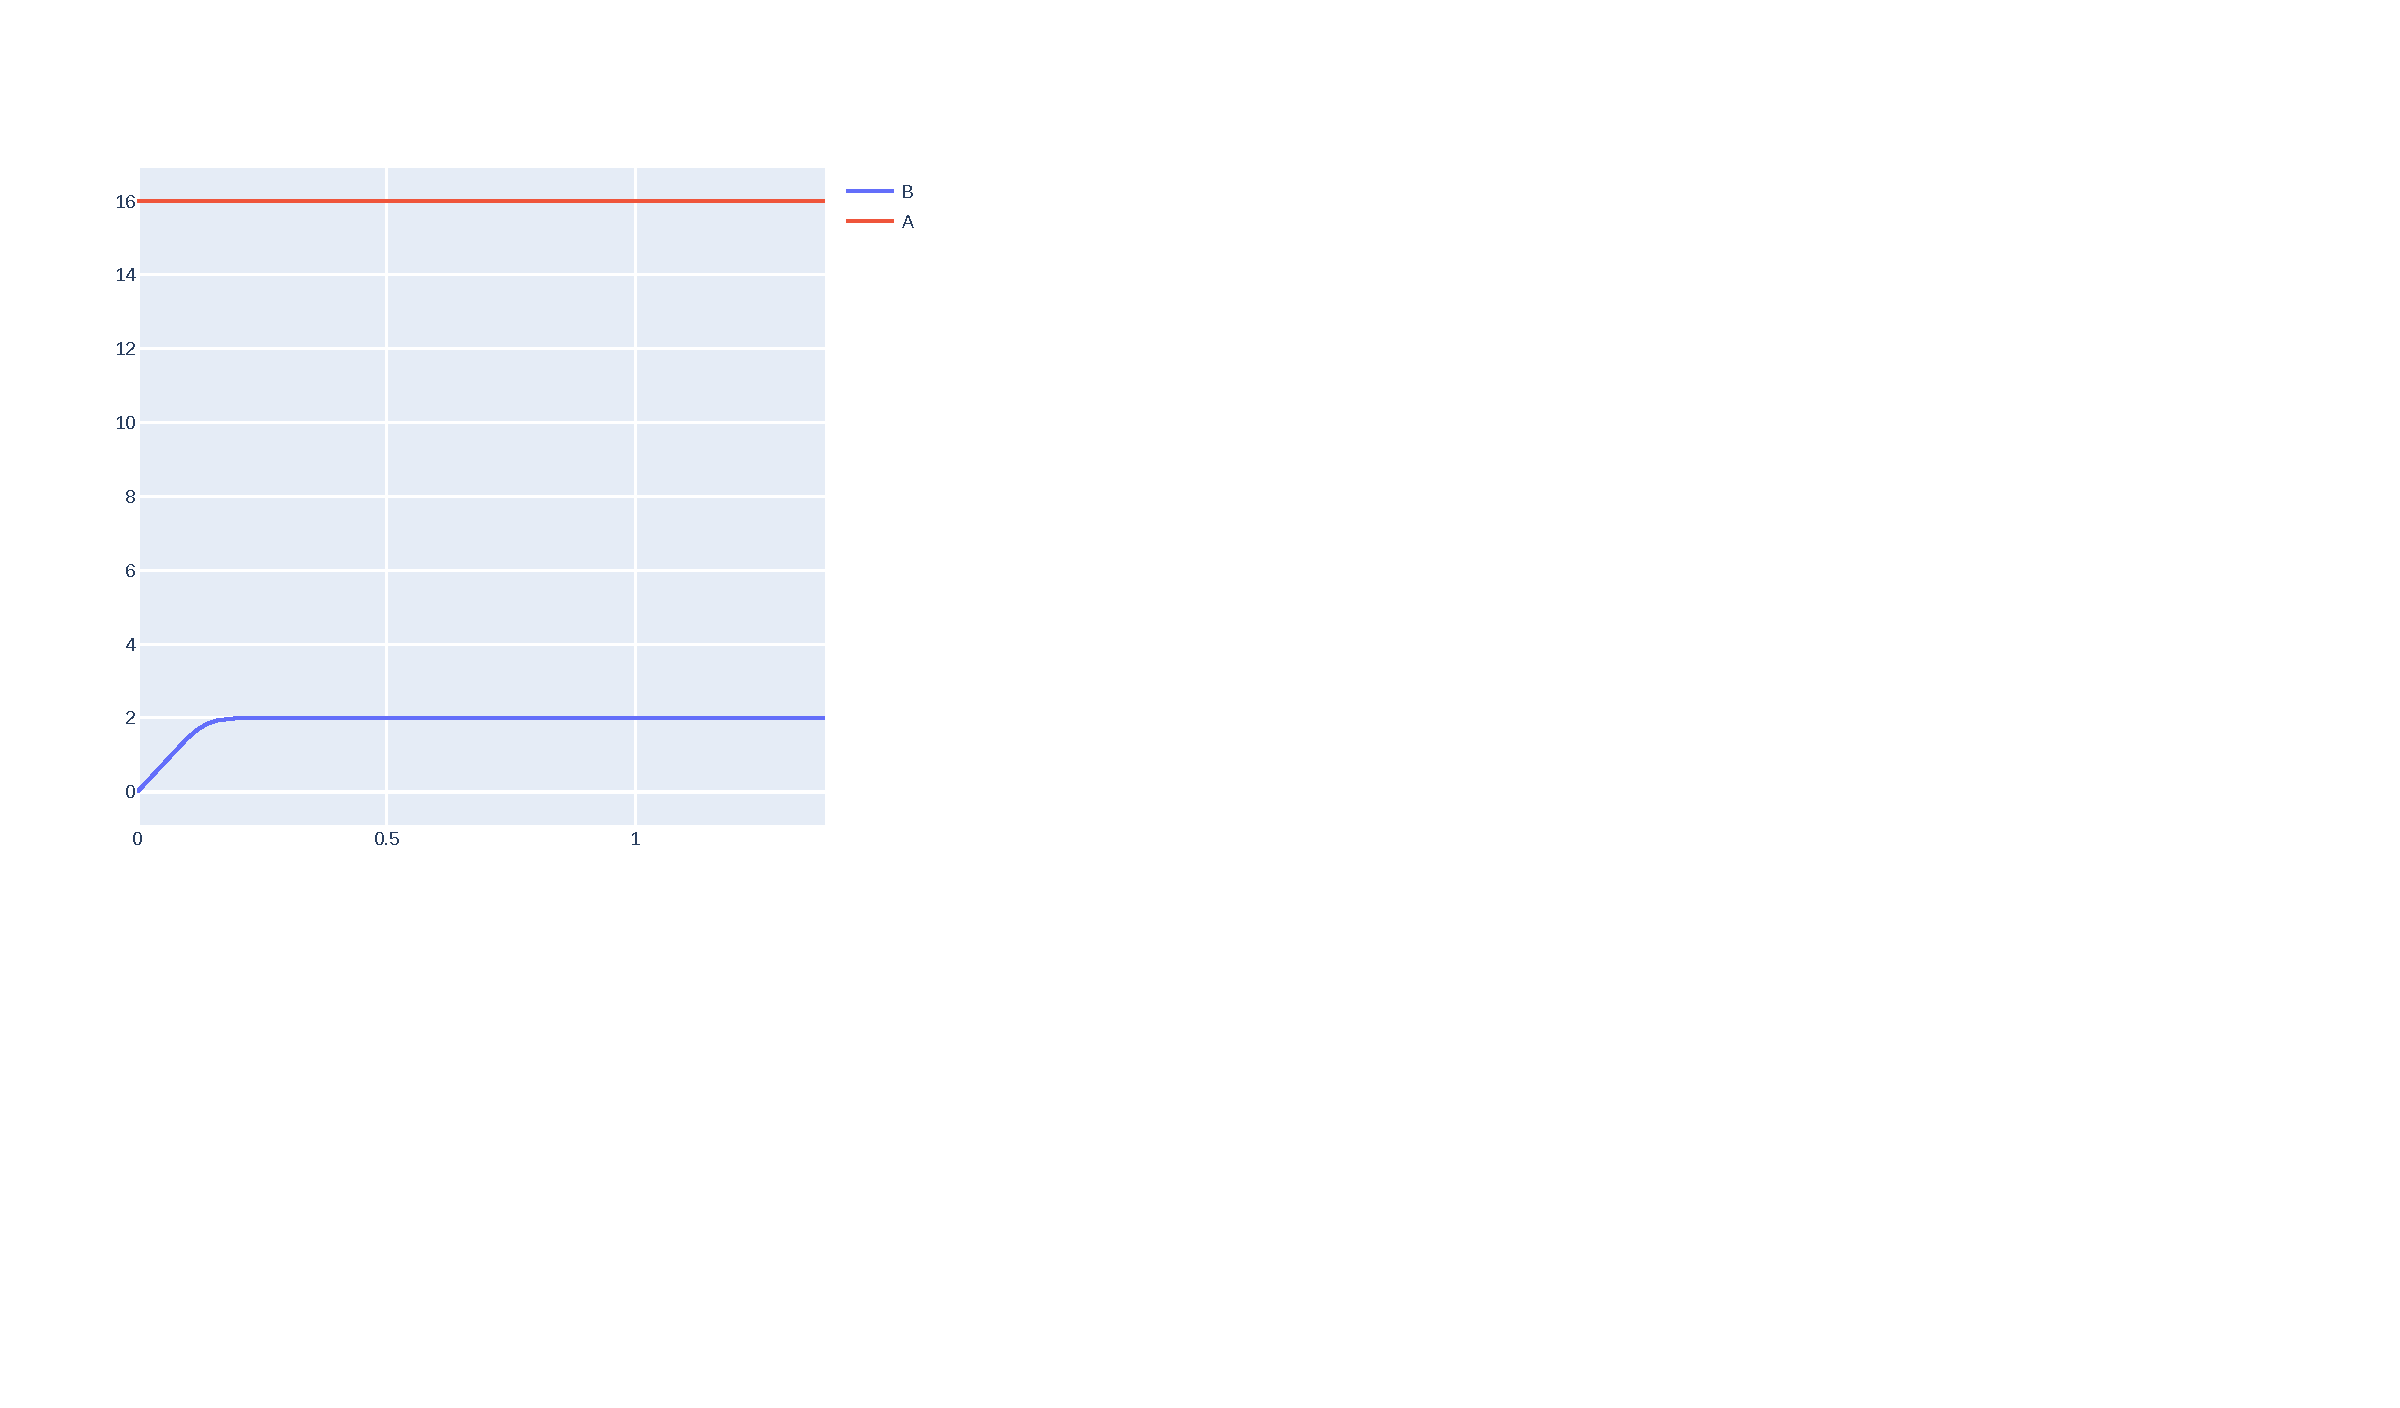
\includegraphics[width=\textwidth]{Figures/sqrt-plot.pdf}
    \caption{\texttt{sqrt[A,B]} resulting in $B=\sqrt[4]{A}$}
    \label{fig:subfigure1}
  \end{subfigure}
  \hfill
  \begin{subfigure}[b]{0.49\textwidth}
    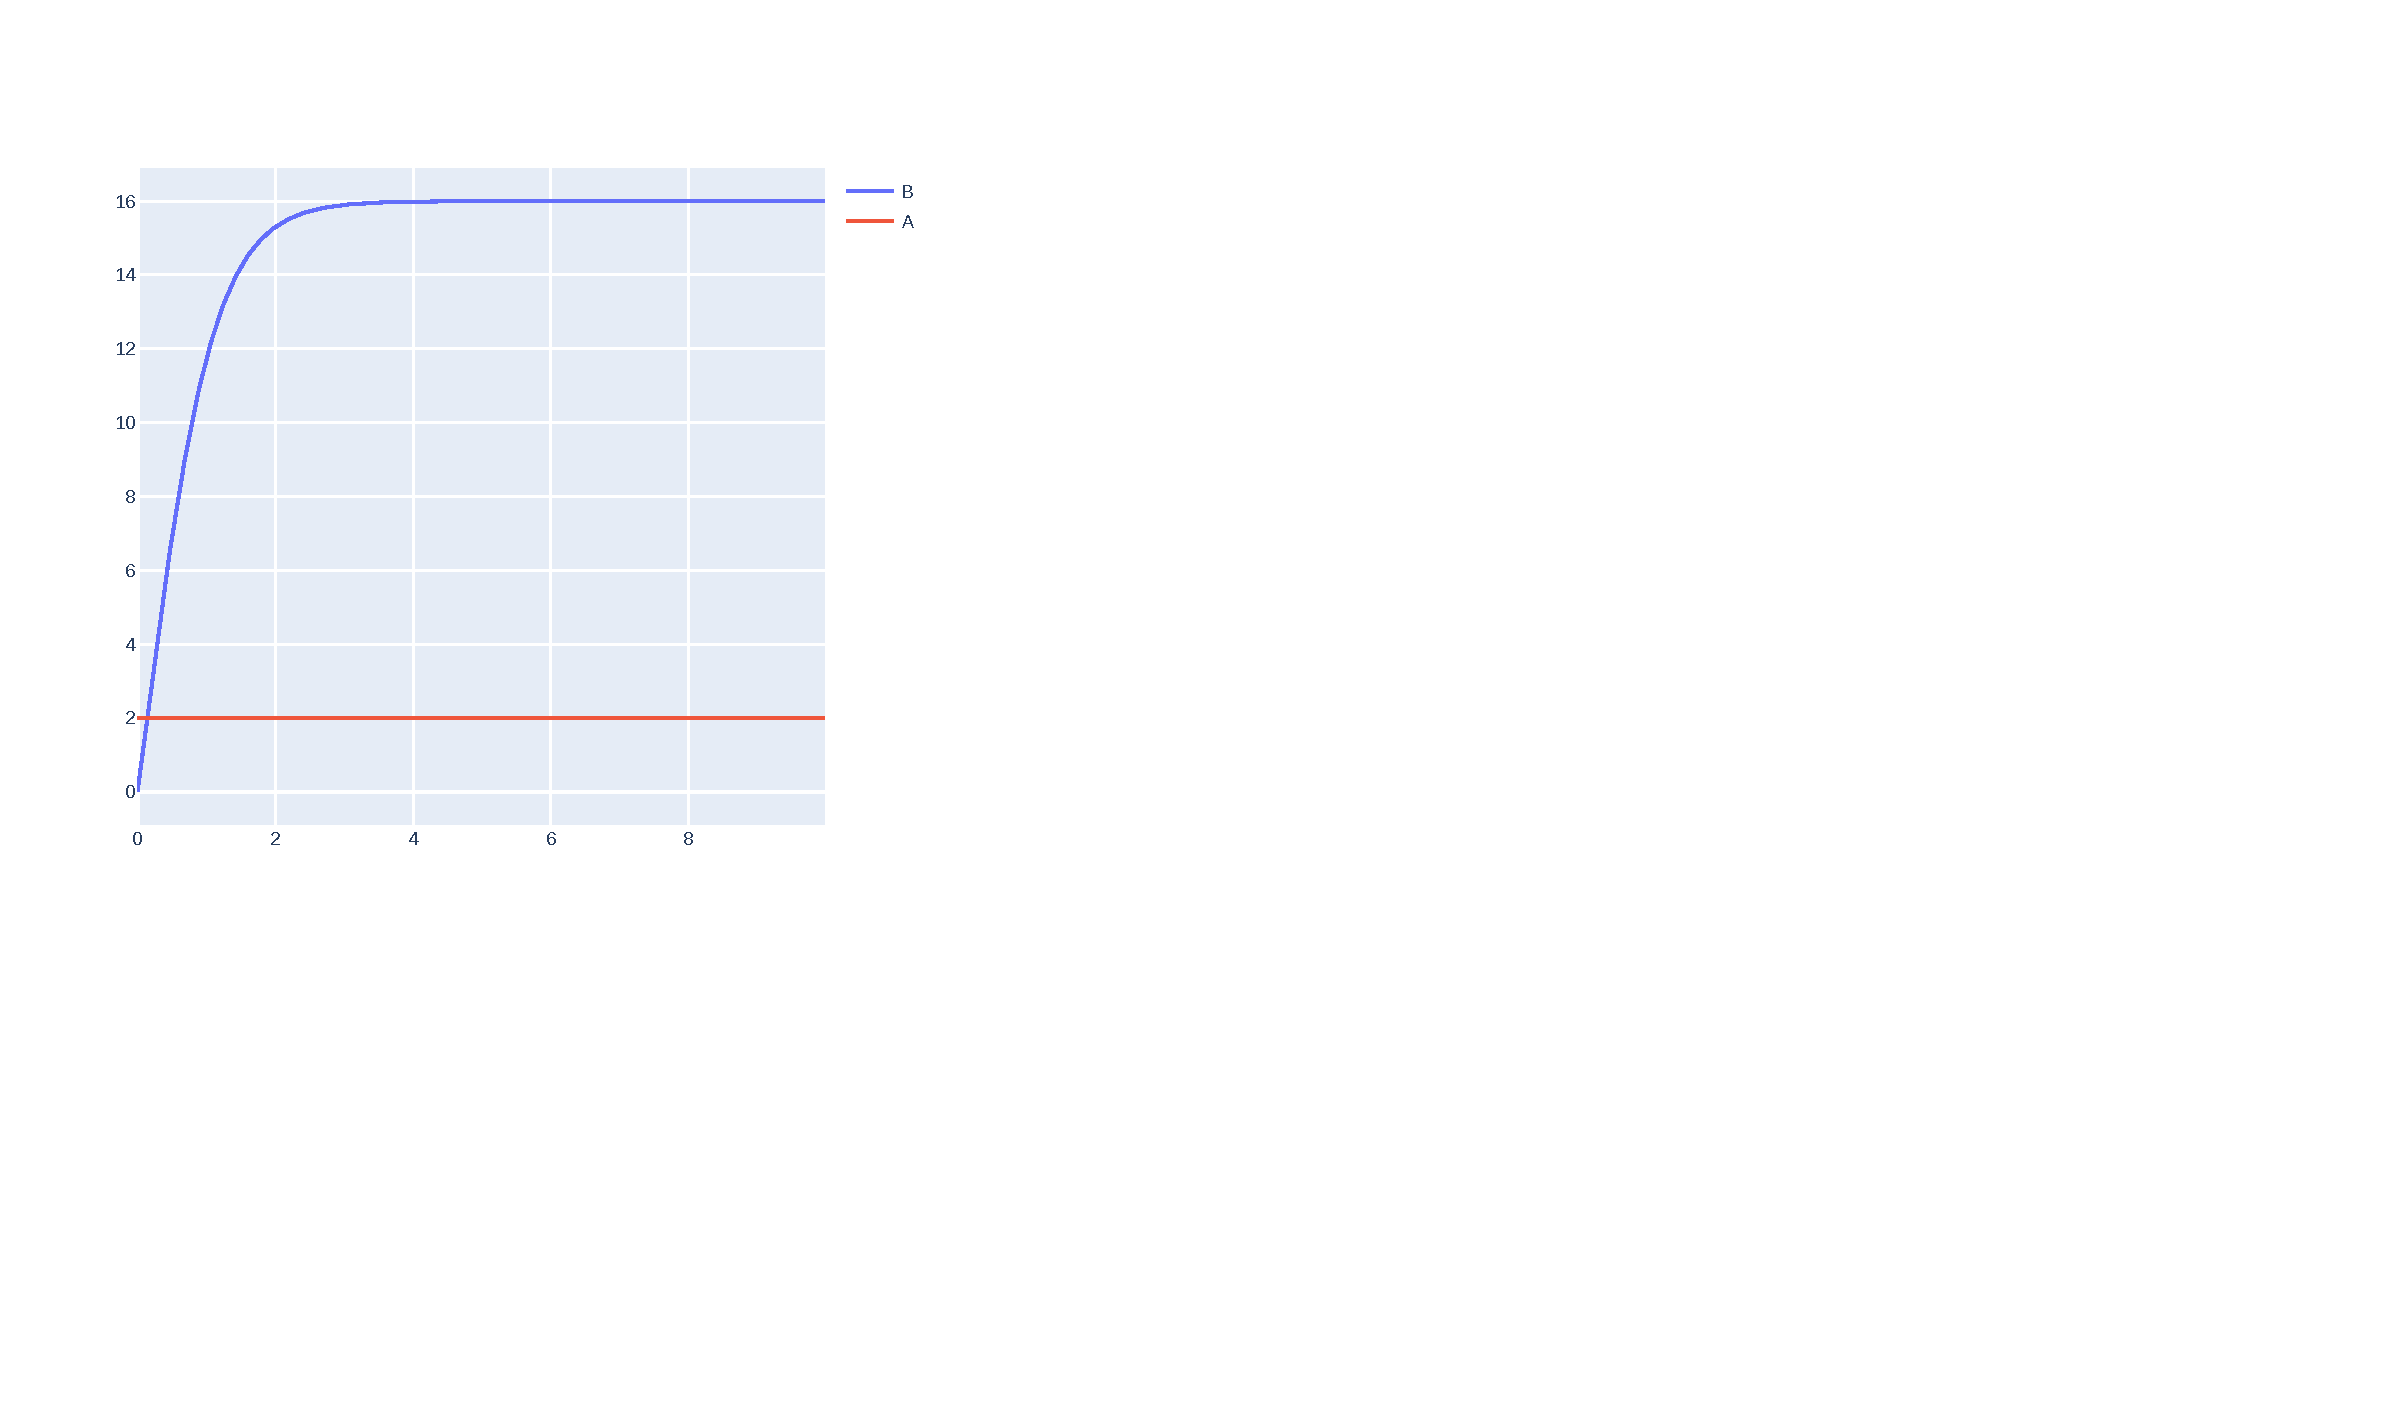
\includegraphics[width=\textwidth]{Figures/mul-plot.pdf}
    \caption{\texttt{mul[A,A,B]} resulting in $B=A^4$}
    \label{fig:subfigure2}
  \end{subfigure}
  \caption{Two showcases of the reaction systems provided in \cite{soloveichik2018a} not providing the correct result.}
  \label{fig:crn-errors}
\end{figure}

Since we have only basic experience in the field of chemistry we resolved to narrowing down our definition of which programs are considered \textit{well-formed} such that they do not allow cases where the reactions do not work properly.

One important aspect of this project is the performance of the simulator. We found the simulation to get out of control for $\mathrm{d}t > 0.04\;\mathrm{s}$. With one clock cycle of the chemical oscillators lasting around a second, this results in a large number of computations even for shorter simulation runs. We tried to optimize all calculations that are part of the simulation as much as possible. For instance, we chose to evaluate the change of each species in one reaction for each reaction instead of the other way around, since this allows us to reuse the product of all concentrations. Another optimization includes to only calculate concentration changes for non-catalysts, i.e. species which have a none-zero net-change.

The generator we built to generate CRNs, could be further optimized like mentioned earlier by not utilizing filtering by predicates and instead only generating \textit{well-formed} CRNs by design. Compared to the time required to simulate multiple steps of a CRN, the time used to generate CRNs is negligible since there is basically no perceivable delay in between successive property based testing iterations.

An attempt was made to use property based testing on the simulator validation function which compares the simulation results with those of the interpreter. With the long time required to simulate the execution of a CRN, this was quickly deemed infeasible though, since only 7 out of 100 tests finished within approximately 10 minutes. Instead, we verified that the property held for all our example CRNs.

%Generator does not produce reliable CRN that can be simulated 